\chapter{Datasets} % Main appendix title

\label{AppendixD} % For referencing this appendix elsewhere, use \ref{AppendixX}

\section{Audi}

The  Audi Autonomous Driving Dataset (A2D2)
authors (\cite{geyer2020a2d2}) are motivated by the fact that research in machine learning, mobile robotics and autonomous driving is accelerated by the availability of high quality annotated data. This statement can be verified by the advances in image classification with deep neural networks since \cite{IMAGENET} became available.  
The A2D2 data was acquired with a human-driven Audi Q7 e-tron equipped with six cameras (front left, front center, front right, back left, back center, back right) and five LiDAR sensors. The authors claim this resulted in  360$^{\circ}$ camera and LiDAR coverage. Additionally, several bus data signals from the vehicle were recorded such as velocity, acceleration and steering wheel angle. 
The total size is 2.3TB. Our datasets of interest are the  Though, since we are interested in image and steering angle only, our data can be narrowed to 
\begin{verbatim}
    https://aev-autonomous-driving-dataset.s3.eu-central-1.amazonaws.com/README-SensorFusion.txt
    
- steering_angle_calculated
- steering_angle_calculated_sign

- 'cam_front_center'
\end{verbatim}

The dataset total size is approximately 2.3TB and provides (...) TBC following https://www.a2d2.audi/a2d2/en/download.html

This was supplied for three cities: Gaimersheim, Ingolstadt and Munich. To perform initial investigations we chose data from Munich and downloaded the "Camera - Front Center" images, constituting 27451 images 3.2MB in size each and dimension 1920x1208 pixels, total size on disk is about 92GB. We also downloaded the 176MB "Bus Signals" file. The image naming convention uses a timestamp in the format:
\begin{verbatim}
20190401145936_camera_frontcenter_000017970.png
\end{verbatim}
The "Bus Signals" file is JSON encoded and provides several signals such as acceleration, angular velocity and vehicle speed. Our signals of interest are the steering angle calculated and steering angle sign. In the bus signals file (20190401121727\_bus\_signals.json) we parsed our values of interest e.g.
\begin{verbatim}
(...)
    "steering_angle_calculated": {
        "unit": "Unit_DegreOfArc",
        "values": [
            [
                1554115464698116,
                2.4
            ],
(...)
\end{verbatim}
where the unit is degree of arc and the values are inferred to be a timestamp when the measurement was acquired and the angle (1554115464698116 and 2.4 respectively, in the example shown).
and found 91968 entries for each of the steering angle and sign. This is over 3 times the amount of corresponding images. Since there was no obvious key to match the steering angle and sign with a corresponding image, we wrote to the supplied enquiry email address aevdrivingdataset@audi.de with regard to this problem and receiving no reply, abandoned the dataset deeming it unusable for our purposes.  
Note: we did try converting the integer into a date using python, which resulted in an error:
\begin{verbatim}
import datetime
audi_timestamp = 1554115464698116
date = datetime.datetime.fromtimestamp(audi_timestamp / 1e3)
print(date)
# ValueError: year 51217 is out of range    
\end{verbatim}

TODO ADD BINS
\begin{figure}[ht]
 \centering 
 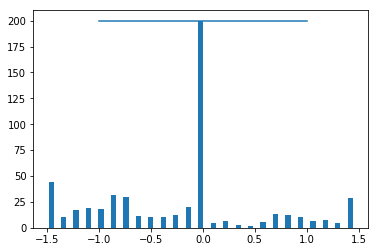
\includegraphics[scale=1]{Figures/bins.png}
 \caption{Diagram showing bins centered around zero degrees, meaning most of time car is driving straight. Binning diagrams for all datasets can be found in appendix B}
 \label{fig:bins-placeholder}
\end{figure}

%% TODO add correspondence with Mentar

\section{Udacity}

1. Link trail - medium (Indian guy) -> medium (Chinese guy)-> github (Japanese guy)  
  
2. Udacity data  
Data is available for download in torrent file format (\cite{torrentCite}) and consist of Robot Operating System (ROS) rosbag compressed files.

\begin{verbatim}
https://github.com/udacity/self-driving-car/tree/master/datasets
\end{verbatim}
3. Rosbag

\section{utbm}
More stuff from german uni?
\begin{verbatim}
https://epan-utbm.github.io/utbm_robocar_dataset/
\end{verbatim}

TODO ADD BINS
\begin{figure}[ht]
 \centering 
 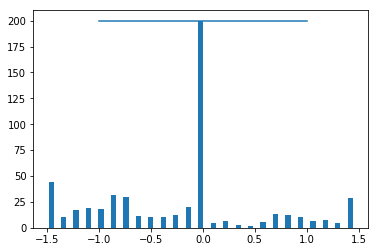
\includegraphics[scale=1]{Figures/bins.png}
 \caption{Diagram showing bins centered around zero degrees, meaning most of time car is driving straight. Binning diagrams for all datasets can be found in appendix B}
 \label{fig:bins-placeholder}
\end{figure}
